% tp2.tex
\documentclass[11pt,a4paper,twocolumn]{article}

% Paramètres de langue et d'encodage
\usepackage[utf8]{inputenc}
\usepackage[T1]{fontenc}
\usepackage[french]{babel}

% Mise en page et marges
\usepackage[margin=1.5cm, top=2.5cm, bottom=2cm, headheight=15pt]{geometry}

% Packages pour les mathématiques, images et tableaux
\usepackage{amsmath,amssymb,amsfonts}
\usepackage{graphicx}
\usepackage{booktabs}
\usepackage{tabularx}
\usepackage{float}
\usepackage{hyperref}
\usepackage{xcolor}
\usepackage{caption}
\usepackage{subcaption}
\usepackage{listings}

% Package pour l'en-tête
\usepackage{fancyhdr}

% Configuration de l'en-tête (s'appliquera après la page de garde)
\pagestyle{fancy}
\fancyhf{}
\fancyhead[L]{USTHB, FGE, ELN}
\fancyhead[C]{4eme GEI}
\fancyhead[R]{TP Communications numériques}
\fancyfoot[C]{\thepage}
\renewcommand{\headrulewidth}{0.4pt}

% Configuration pour le code source Python
\lstset{
  language=Python,
  basicstyle=\scriptsize\ttfamily,
  keywordstyle=\bfseries,
  stringstyle=\color{darkgray},
  commentstyle=\color{gray}\itshape,
  numbers=left,
  numberstyle=\tiny\color{gray},
  frame=single,
  breaklines=true,
  showstringspaces=false,
  tabsize=4
}

\begin{document}

% ==========================================
% PAGE DE GARDE (Uniquement sur une colonne)
% ==========================================
\begin{titlepage}
    % Les logos et l'en-tête de l'université
    \noindent
    \begin{minipage}{0.18\textwidth}
        
\includegraphics[width=\linewidth]{usthb.png}
    \end{minipage}
    \hfill
    \begin{minipage}{0.6\textwidth}
        \centering
        \small
        République Algérienne Démocratique et Populaire\\
        Ministère de l'enseignement Supérieur et de la Recherche Scientifique\\
        Université des Sciences et de la Technologie Houari Boumediene\\[0.3cm]
        \textbf{\large Faculté Génie Electrique}\\[0.1cm]
        \textbf{\large Département d'électronique}
    \end{minipage}
    \hfill
    \begin{minipage}{0.18\textwidth}
        \raggedleft
        
\includegraphics[width=\linewidth]{fge.png}
    \end{minipage}

    \vspace{2cm}

    % Niveau d'étude
    \begin{center}
        \textbf{\Large 4\textsuperscript{éme} Année Ingénieur}\\[0.2cm]
        \textbf{\Large Électronique Industrielle}
    \end{center}

    \vspace{2cm}

    % Titre principal
    \begin{center}
        \textbf{\Huge Travaux Pratiques}\\[0.8cm]
        \textbf{\LARGE COMMUNICATIONS NUMÉRIQUES}\\[0.8cm]
        \Large Compte rendu № 3\\[0.5cm]
        \Large Date : \today
    \end{center}

    \vspace{1.5cm}

    % Encadré avec l'intitulé du TP
    \begin{center}
        \framebox[\textwidth]{
            \begin{minipage}{0.9\textwidth}
                \vspace{0.4cm}
                \begin{center}
                    \huge \textbf{Intitulé du TP : Modulations numériques}
                \end{center}
                \vspace{0.4cm}
            \end{minipage}
        }
    \end{center}

    \vspace{2.5cm}

    % Informations des étudiants
    \begin{flushleft}
        \Large
        \textbf{Nom et Prénoms de l'étudiant 1 :} Hachemi Rahim Wassim\\[0.4cm]
        \textbf{Nom et Prénoms de l'étudiant 2 :} Tedjoui Abdelmalek\\[0.4cm]
        \textbf{Sous-groupe :} 5\\[0.4cm]
        \textbf{E-mail :} \texttt{wrhachemi@gmail.com}
    \end{flushleft}

\end{titlepage}
% ==========================================
% FIN DE LA PAGE DE GARDE
% ==========================================

\vspace*{0.3cm}
\begin{center}
\textbf{\large TP3 : Modulations numériques}
\end{center}

\section*{Introduction}
Ce compte rendu présente l'étude et la mise en oeuvre de plusieurs schémas de modulation numérique demandés dans le TP3. L'objectif est d'implémenter des modulateurs élémentaires (ASK/OOK, BPSK, QPSK, 16-QAM, 64-QAM), d'analyser leurs constellations en présence de bruit et de comparer l'effet du rapport signal-à-bruit en énergie par bit (Eb/N0).

\section*{Rappel théorique}
Pour une modulation numérique, chaque symbole transporte un nombre de bits égal à $\log_2(M)$ où $M$ désigne le nombre de points de la constellation. Les modulations à faible ordre, comme ASK/OOK et BPSK, offrent une meilleure robustesse au bruit mais une efficacité spectrale plus faible. À l'inverse, les modulations QAM d'ordre élevé améliorent le débit utile à bande passante fixée, au prix d'une séparation plus faible entre symboles.

Dans le script, les symboles de QAM sont normalisés afin que l'énergie moyenne reste comparable entre les constellations. Cela permet d'étudier l'effet du bruit sans que les différences observées viennent seulement de l'échelle des amplitudes.

\section*{Méthodologie}
La simulation est réalisée en Python dans le fichier \texttt{modulations\_numeriques.py}. Les paramètres principaux sont : débit binaire $R_b=1000\,$Hz, fréquence porteuse $f_c=4000\,$Hz, fréquence d'échantillonnage $f_s=32000\,$Hz et une séquence de $1000$ bits. Les figures incluses ont été générées par le script et sauvegardées en PNG.

\section*{Extraits de code essentiels}
Les extraits ci-dessous montrent la définition de la classe de simulation et les fonctions d'ajout de bruit (réutilisées pour générer les constellations bruitées).

\begin{lstlisting}
class ModulationNumerique:
    def __init__(self, EbN0_dB=10):
        self.Rb = 1000
        self.fc = 4000
        self.fs = 32000
        self.Nbits = 1000
        self.EbN0_dB = EbN0_dB
        self.Ns = int(self.fs / self.Rb)

        np.random.seed(42)
        self.bits = np.random.randint(0, 2, self.Nbits)

        self.t = np.arange(0, self.Nbits/self.Rb, 1/self.fs)
        self.port_cos = np.sqrt(2) * np.cos(2 * np.pi * self.fc * self.t)
        self.port_sin = np.sqrt(2) * np.sin(2 * np.pi * self.fc * self.t)
        self.noms_modulations = ['ASK/OOK', 'BPSK', 'QPSK', '16-QAM', '64-QAM']
\end{lstlisting}

\begin{lstlisting}
    def ajouter_bruit_symboles(self, symboles, EbN0_dB=None):
        if EbN0_dB is None:
            EbN0_dB = self.EbN0_dB
        EbN0 = 10**(EbN0_dB / 10)
        Es = np.mean(np.abs(symboles)**2)
        M = len(np.unique(symboles))
        Eb = Es / np.log2(M)
        N0 = Eb / EbN0
        if np.isreal(symboles).all():
            bruit = np.sqrt(N0/2) * np.random.randn(len(symboles))
        else:
            bruit = np.sqrt(N0/2) * (np.random.randn(len(symboles)) + \
                                    1j * np.random.randn(len(symboles)))
        return symboles + bruit
\end{lstlisting}

Ces extraits sont suffisants pour comprendre la façon dont le bruit est appliqué aux symboles et comment les paramètres de base sont définis.

\section*{Résultats}
Les figures suivantes résument les résultats demandés : signaux modulés dans le domaine temporel et constellations bruitées pour différents niveaux d'Eb/N0. Les images ont été générées par le script fourni.

La première figure montre que les modulations ASK/OOK et BPSK sont directement visibles par alternance d'amplitude ou de signe sur la porteuse, alors que les modulations en quadrature présentent une combinaison des composantes I et Q. Cette étape sert surtout à vérifier que les signaux sont bien construits avant d'étudier les constellations.

\begin{figure*}[t]
\centering
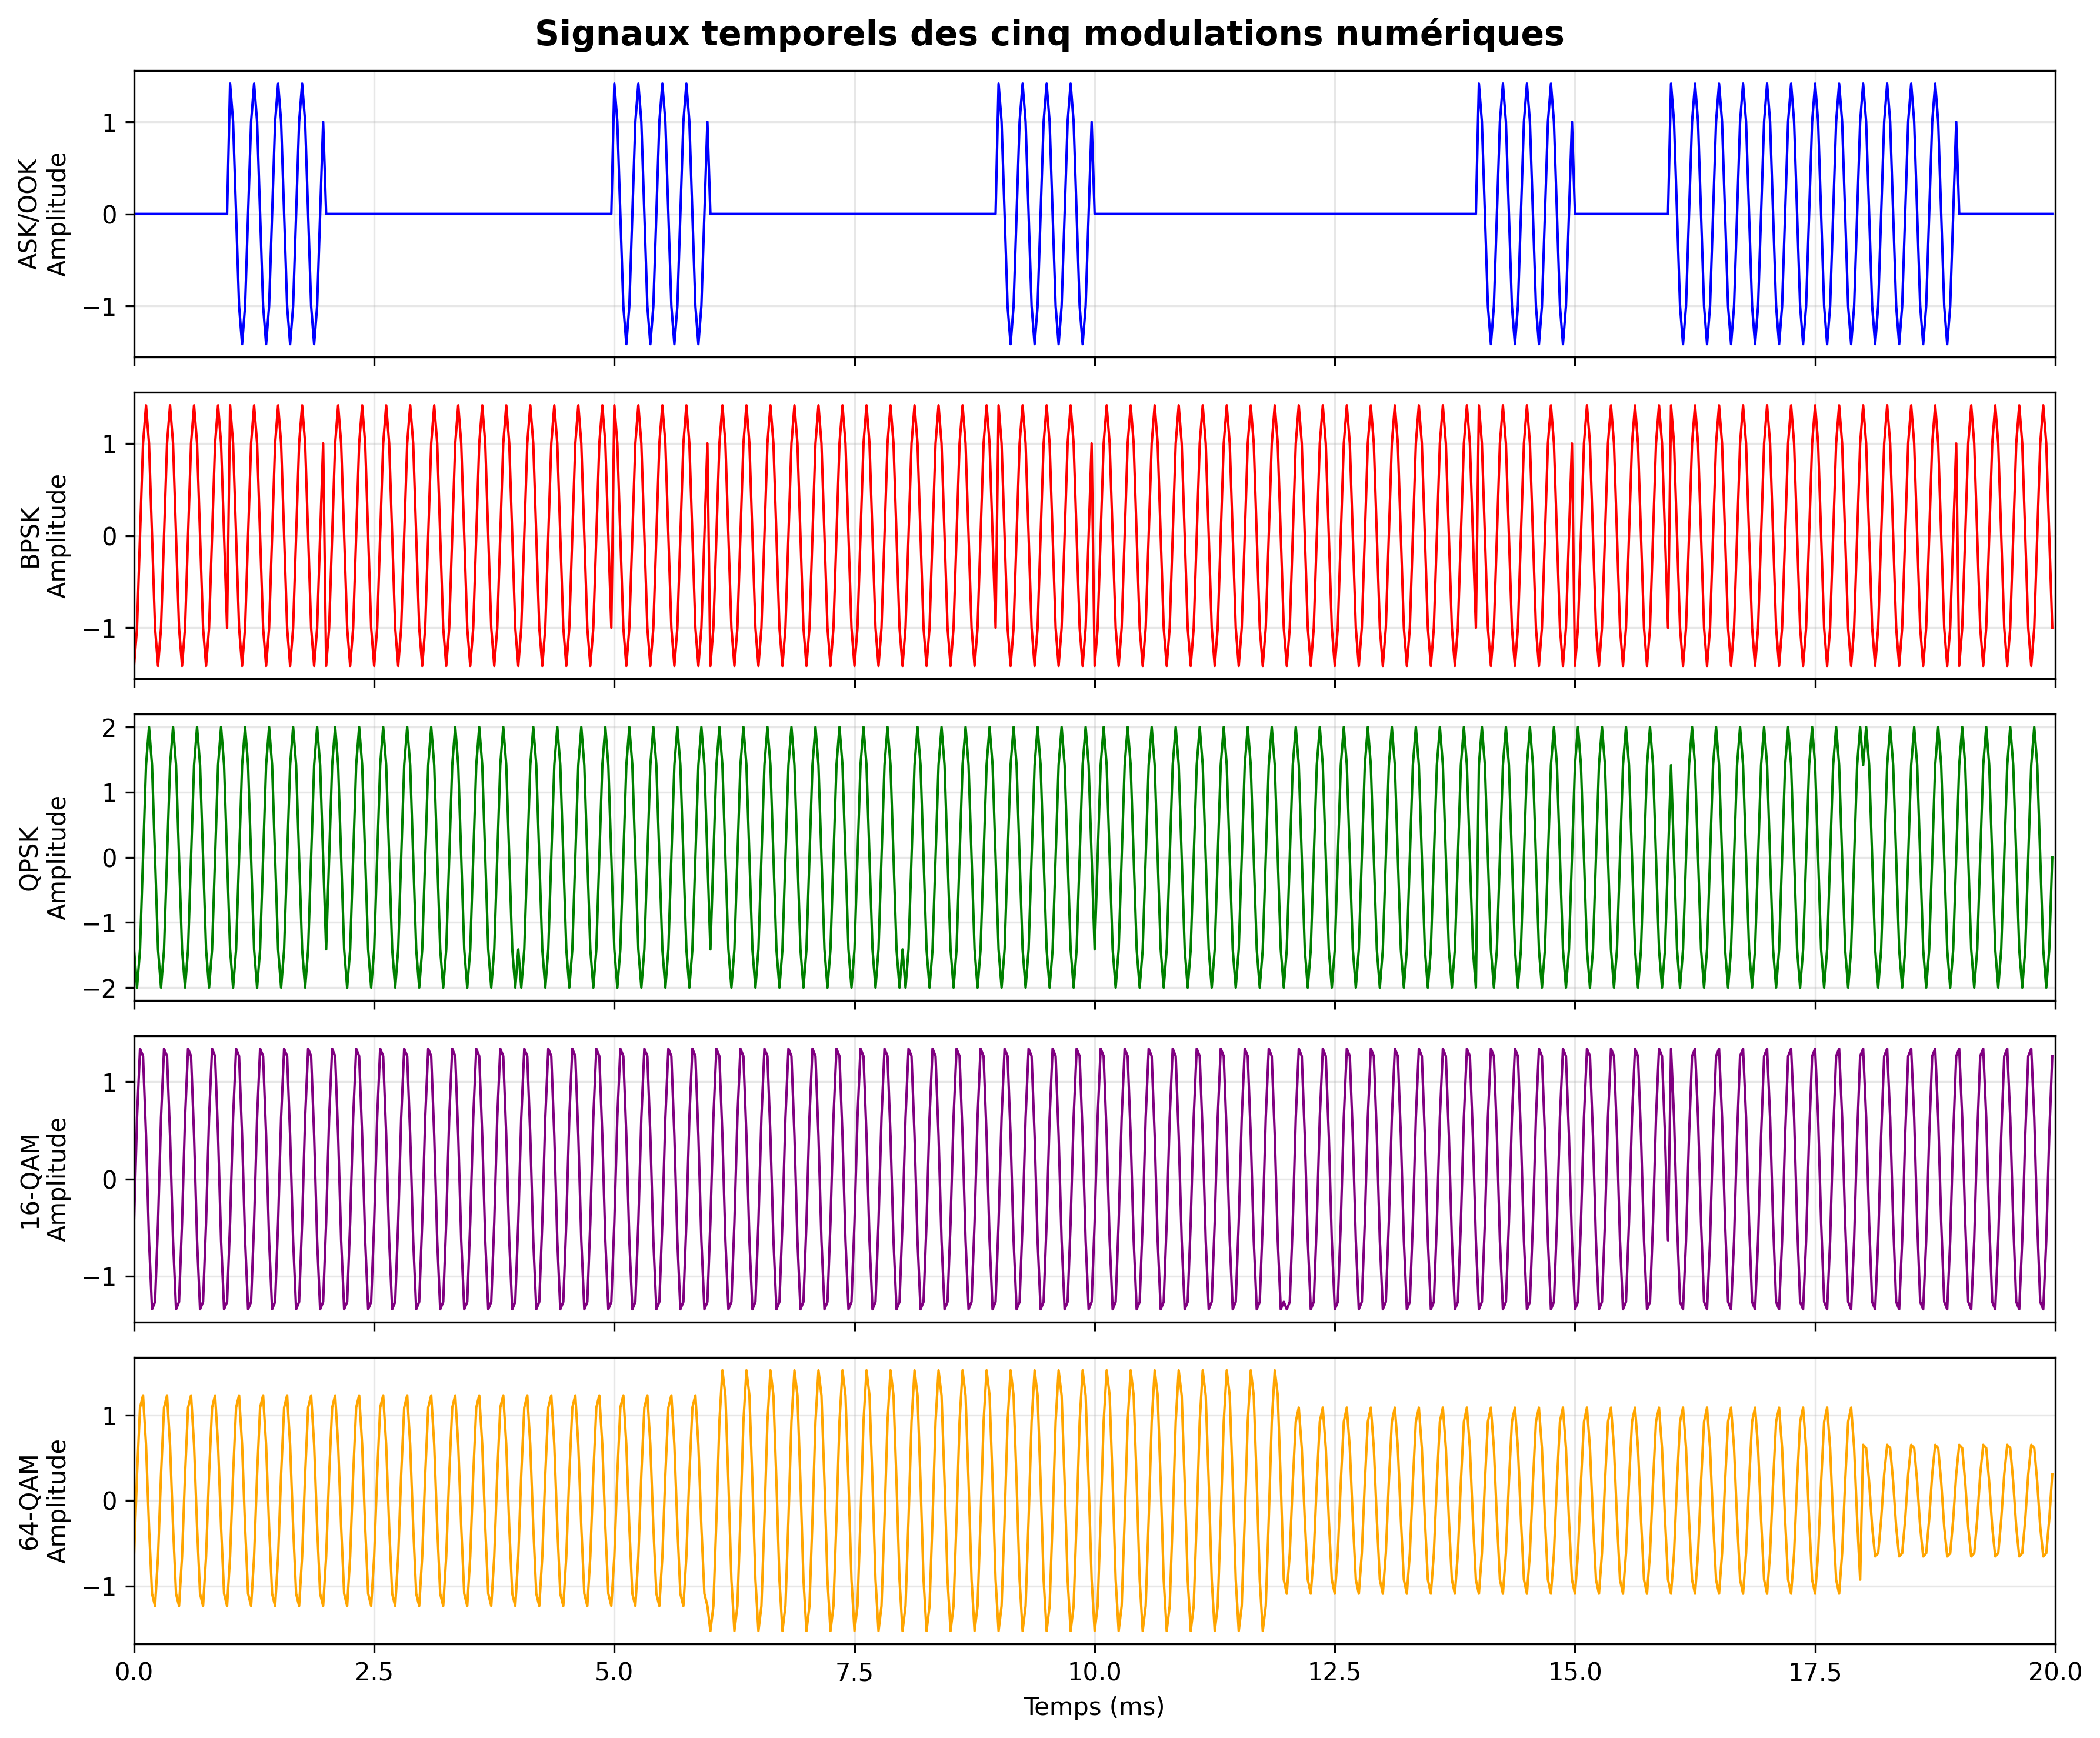
\includegraphics[width=0.95\textwidth]{01_signaux_modules.png}
\caption{Signaux modulés (fenêtre temporelle de 20 bits) pour les cinq modulations étudiées.}
\end{figure*}

Les constellations bruitées permettent de visualiser la sensibilité de chaque modulation. Pour Eb/N0 faible, les points se recouvrent davantage et les zones de décision deviennent incertaines. Pour Eb/N0 plus élevé, les nuages de points se recentrent autour des symboles idéaux.

\begin{figure*}[t]
\centering
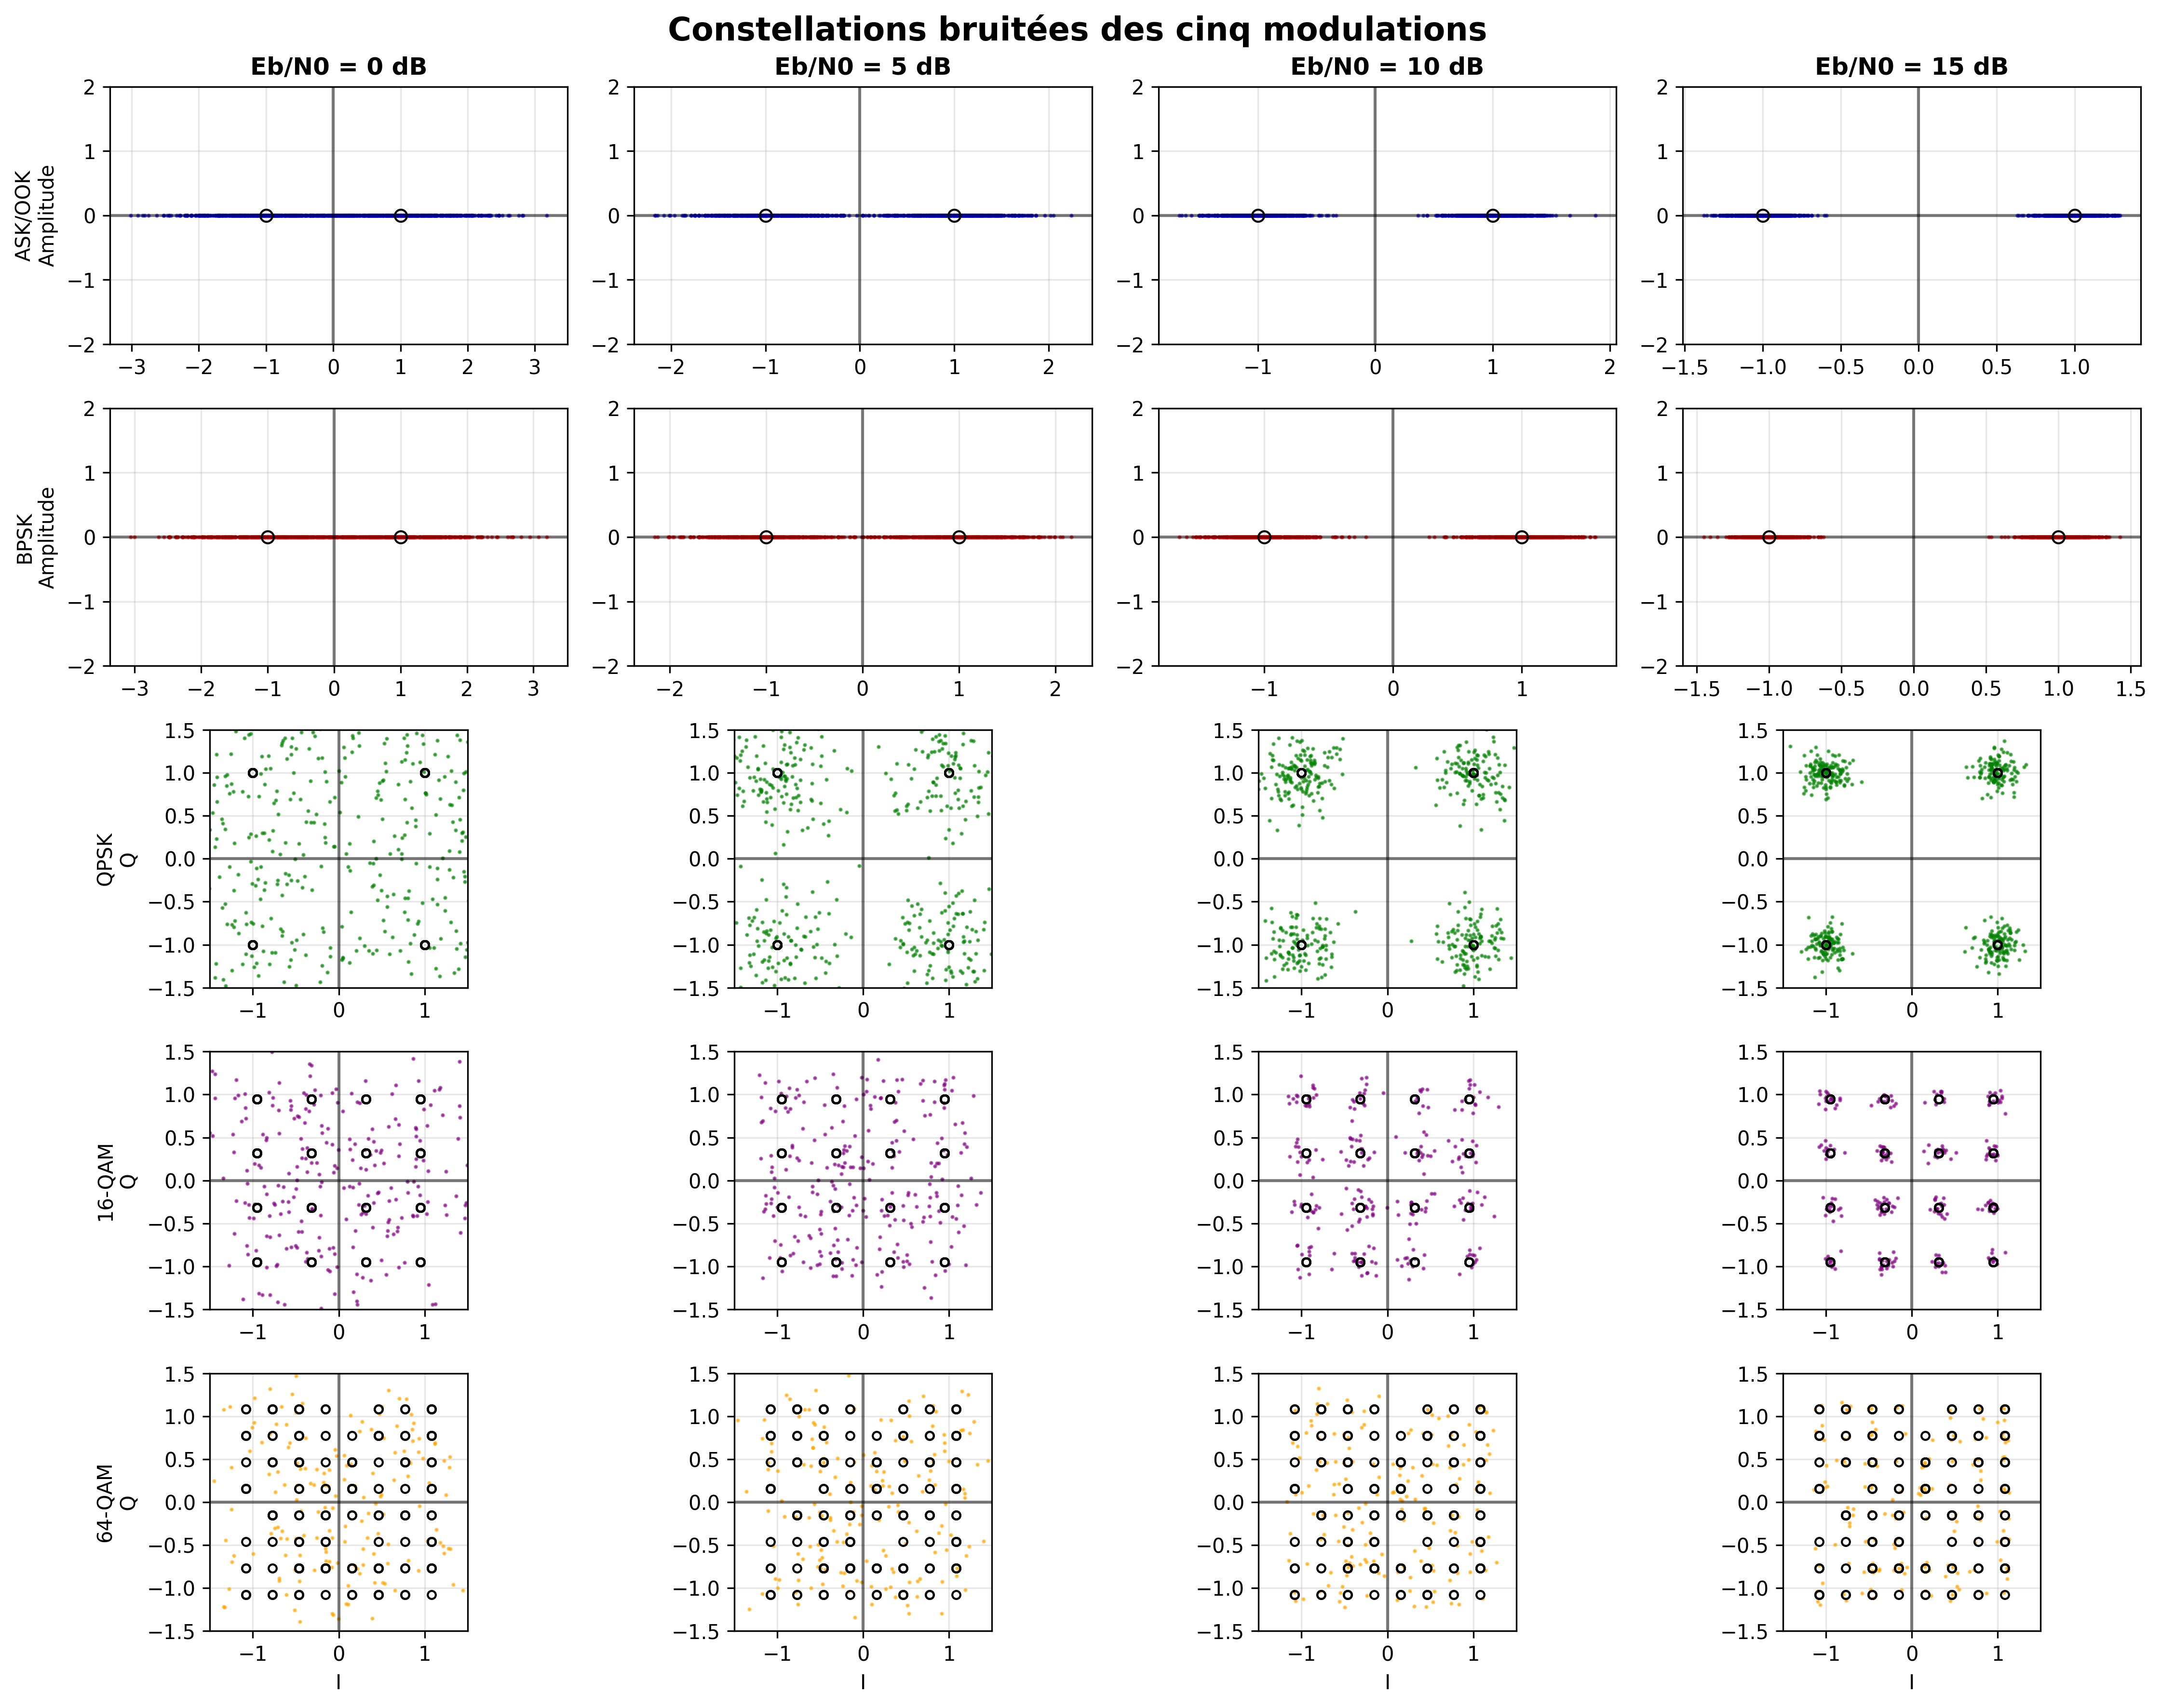
\includegraphics[width=0.95\textwidth]{02_constellations_bruit.png}
\caption{Constellations bruitées pour Eb/N0 = 0, 5, 10, 15 dB (colonnes). Chaque ligne correspond à une modulation.}
\end{figure*}

La comparaison finale confirme que les modulations à grand nombre d'états sont les plus fragiles. À titre d'exemple, le 64-QAM garde une bonne efficacité spectrale, mais il exige un canal plus propre que le BPSK ou le QPSK. Cette différence est exactement celle que l'on attend en communications numériques.

\begin{figure*}[t]
\centering
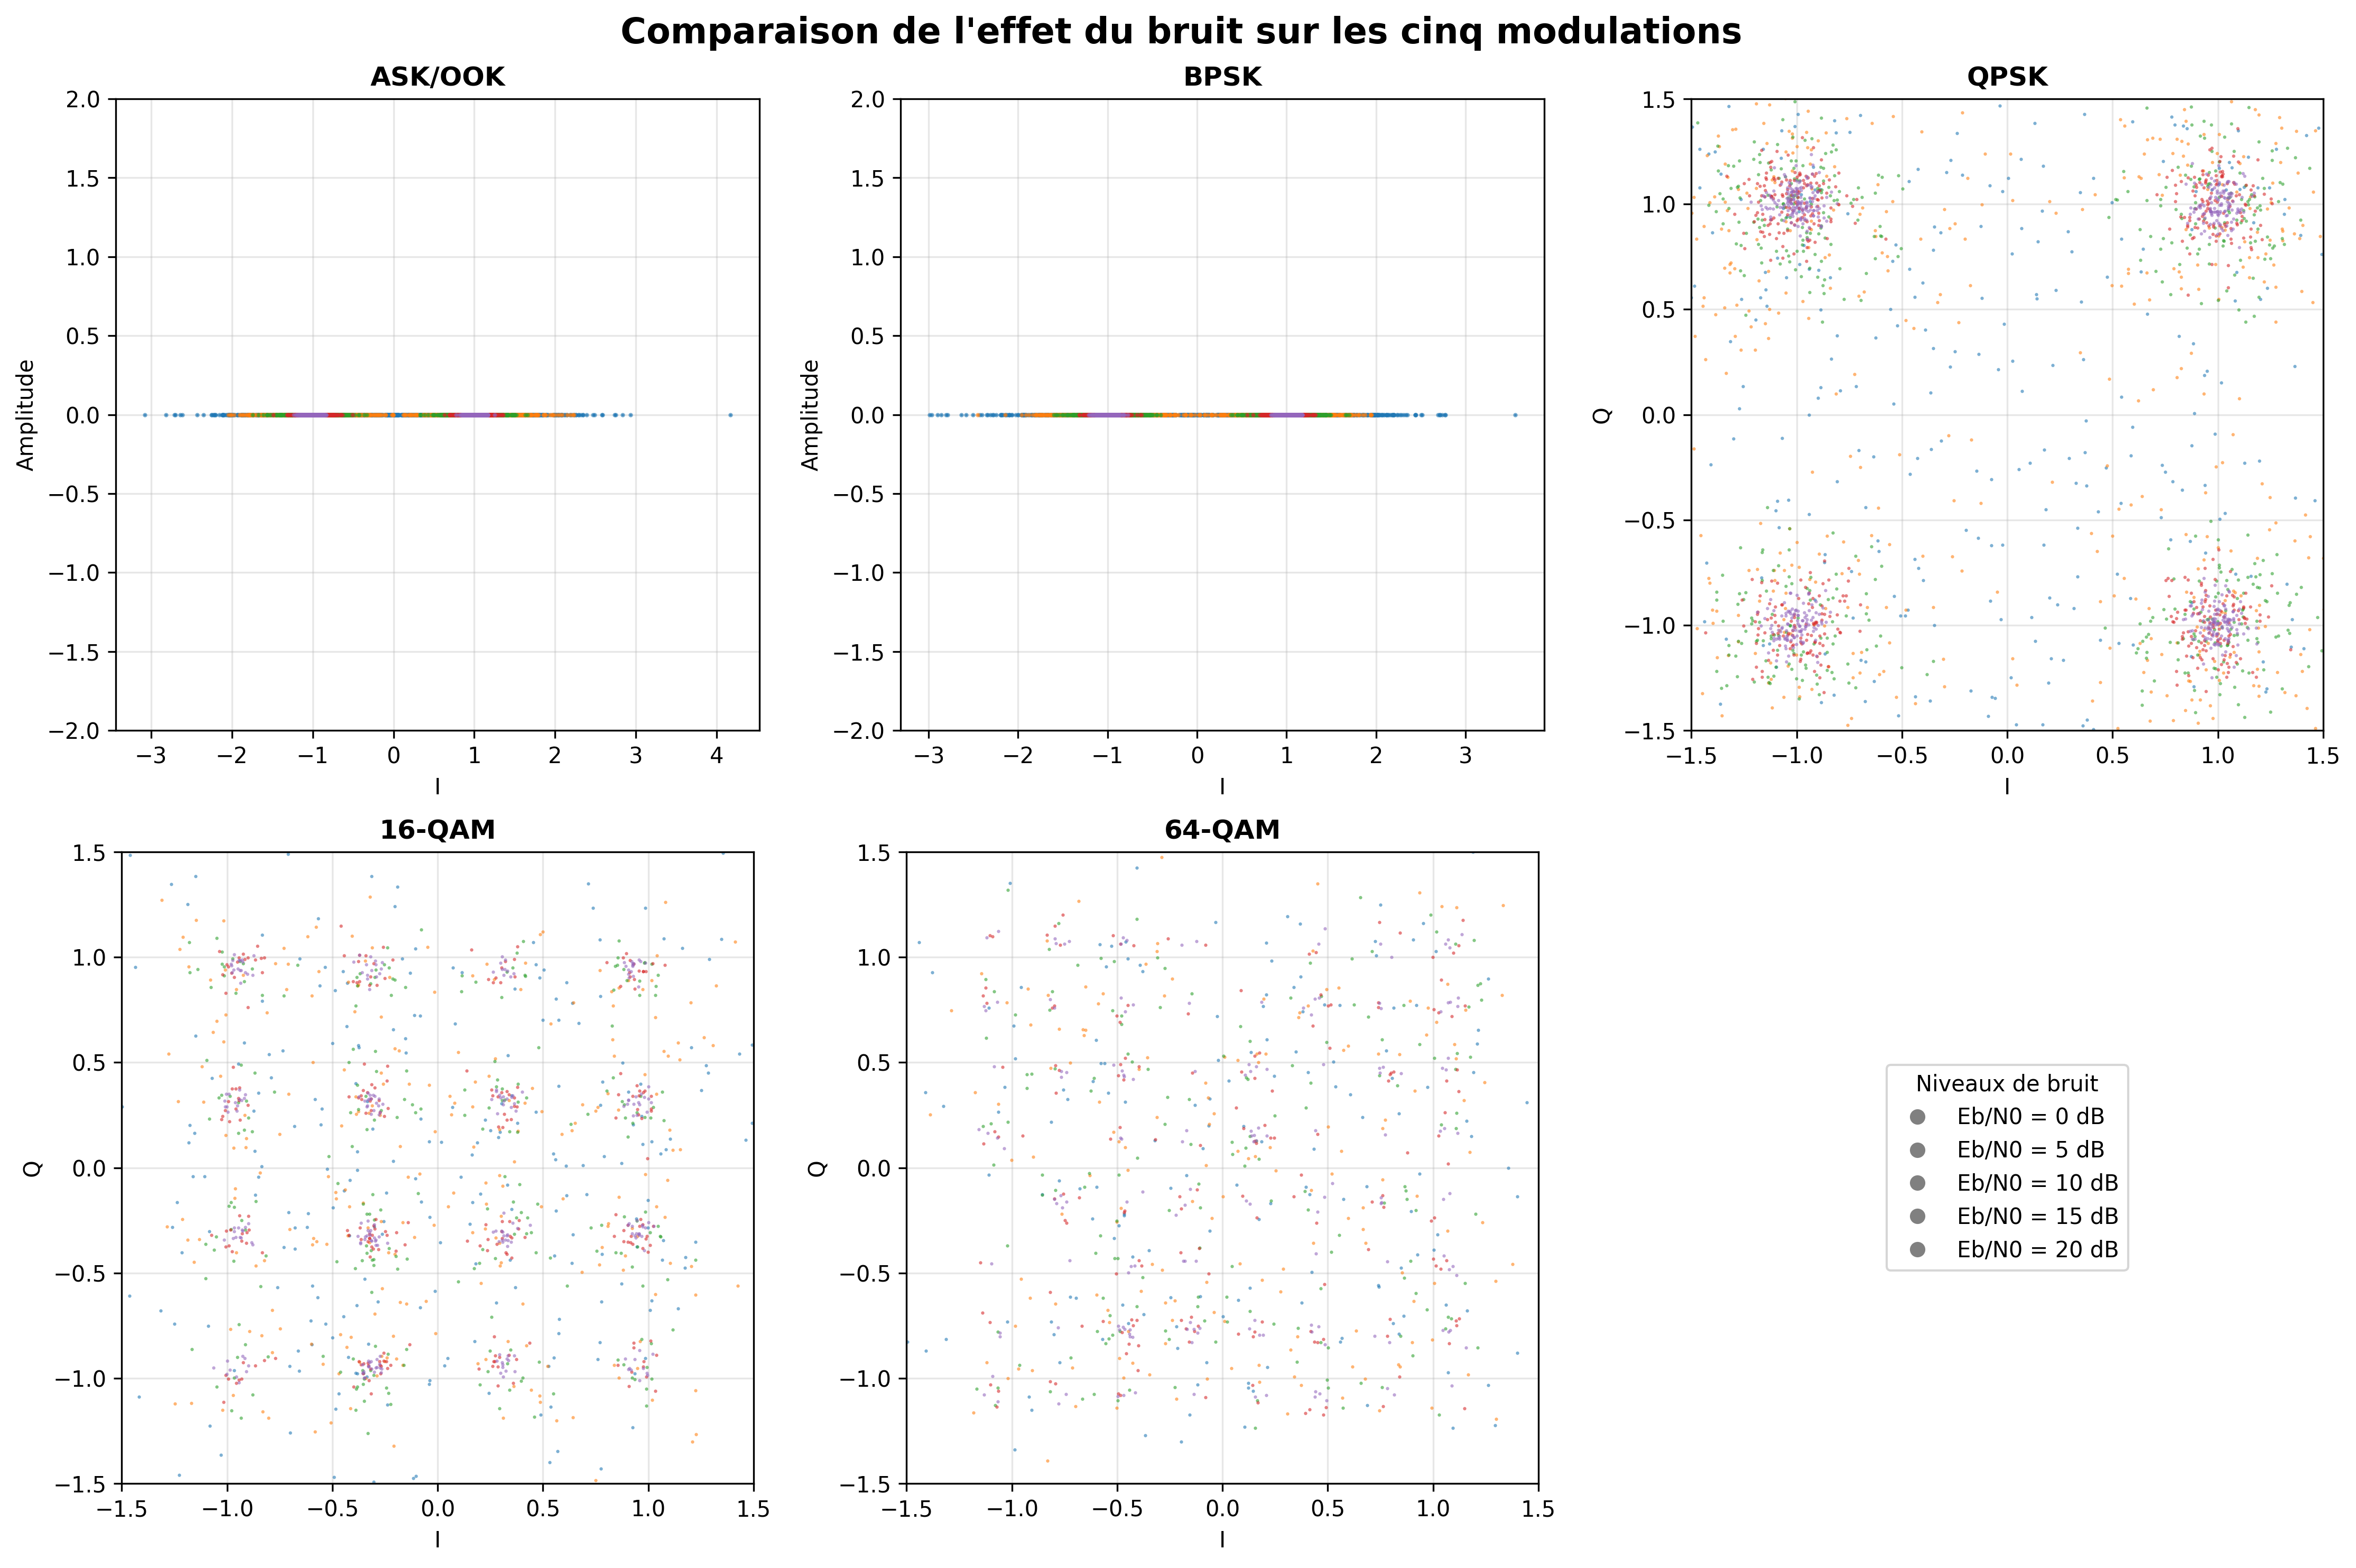
\includegraphics[width=0.95\textwidth]{03_comparaison_bruit.png}
\caption{Comparaison de l'effet du bruit sur les modulations pour plusieurs valeurs d'Eb/N0.}
\end{figure*}

\section*{Analyse et réponses aux questions}
Les correspondances obtenues sont : ASK/OOK pour la première modulation, BPSK pour la deuxième, QPSK pour la troisième, 16-QAM pour la quatrième et 64-QAM pour la cinquième. Cette identification est cohérente avec le nombre de points de constellation et avec la structure de la modulation dans le domaine temporel.

L'effet du bruit est très visible sur les constellations : pour Eb/N0 faible, les points se dispersent autour de leurs positions idéales et les nuages deviennent plus difficiles à séparer. Quand Eb/N0 augmente, les symboles se resserrent et les frontières de décision deviennent plus nettes. Le phénomène est plus marqué pour 16-QAM et 64-QAM, car l'écart entre points voisins est plus petit que pour BPSK ou QPSK.

Sur les signaux temporels, on remarque aussi que les modulations à amplitude variable présentent des enveloppes plus contrastées. ASK/OOK utilise directement la présence ou l'absence de porteuse, alors que BPSK change seulement le signe de la porteuse. Les QAM combinent les composantes en phase et en quadrature, ce qui explique la densité plus importante des points sur le plan I/Q.

En pratique, les figures confirment que la montée en ordre de modulation améliore la quantité d'information transmise par symbole, mais dégrade la tolérance au bruit. Le choix d'une modulation dépend donc du compromis entre robustesse, débit et largeur de bande disponible.

Une autre observation est que le bruit ajouté dans le script est gaussien et indépendant sur les composantes réelle et imaginaire pour les symboles complexes. Cela correspond bien au modèle classique de canal AWGN utilisé dans les premiers travaux pratiques de communication numérique.

\section*{Conclusion}
Le TP a permis de vérifier expérimentalement les différences de robustesse au bruit entre schémas de modulation et de se familiariser avec la simulation temps-fréquence et l'affichage des constellations. Le code fourni est suffisant pour reproduire les expériences et peut être étendu pour estimer le taux d'erreur binaire (BER) empirique.

\end{document}
